\documentclass[12pt,a4paper]{article}
\usepackage{styles}

\lstset{style=sharpc, tabsize=1}


\author{Alexander van Schie \& Oli Dias}
\title{Gruppenarbeit 1 - Cloud Fundamentals beim Provider}
\begin{document}
\maketitle
\newpage
\tableofcontents
\newpage
\section{Hands-On: Hello (Cloud) World}
%TODO Einleitung schreiben mit erklärung wieso, Start Stopp Möglichkeiten, Logfiles, Vorteil/Nachteil ggü Google App Engine
\subsection{Installationsanleitung}
Das Ziel ist es, eine Asp.Net-Core Hello-World Applikation mittels Openshift Online zu builden und deployen. Am Schluss dieser Installationsanleitung sollte dies möglich sein.


Für das Einrichten von Openshift Online müssen grob folgende Schritte durchgeführt werden:
\begin{itemize}
	\item Account und Projekt auf der Plattform erstellen
	\item GitHub Repository der Asp.Net-Core Applikation mit Openshift Projekt verbinden
	\item Applikation auf Openshift builden
	\item Applikation auf Openshift deployen
\end{itemize}
\subsubsection{Openshift Account erstellen}
Zuerst muss ein Account auf  \url{https://manage.openshift.com/signin} erstellt werden. Danach kann zwischen den in Abbildung \ref{fig:openshift-plan} vorgeschlagenen Plänen ausgewählt werden. Wir benutzen den Openshift Online Starter Plan.
\begin{figure}[h]
	\centering
	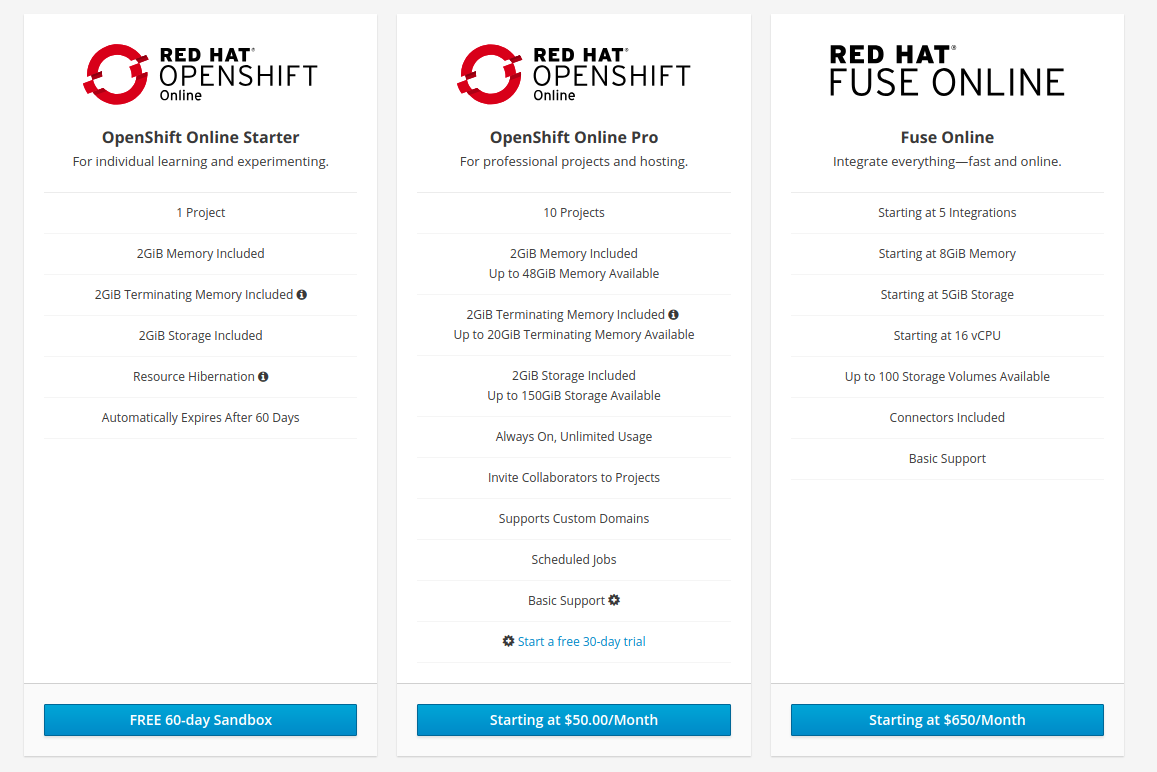
\includegraphics[width=0.7\linewidth]{img/openshift-plan}
	\caption{Gewählter Plan Openshift}
	\label{fig:openshift-plan}
\end{figure}

Dass der Account verifiziert werden kann, muss eine Telefonnummer hinterlegt werden, auf welche darauffolgend einen Bestätigungscode zugeschickt wird. 
\begin{figure}[h]
	\centering
	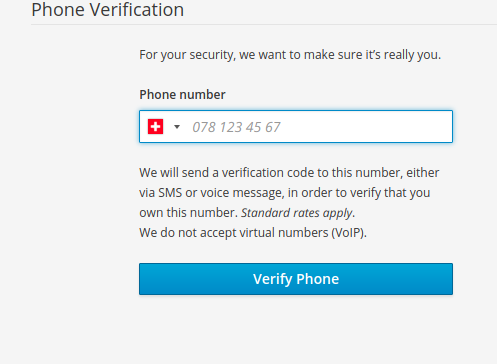
\includegraphics[width=0.7\linewidth]{img/os-phone-validation}
	\caption{Telefon Verifikation}
	\label{fig:os-phone-validation}
\end{figure}
Wurde diese eingegeben und verifiziert, erscheint eine Übersicht über das bestellte Produkt wie in Abbildung \ref{fig:os-overview} angezeigt. Daraufhin kann die Subscription bestätigt werden.
\begin{figure}[h]
	\centering
	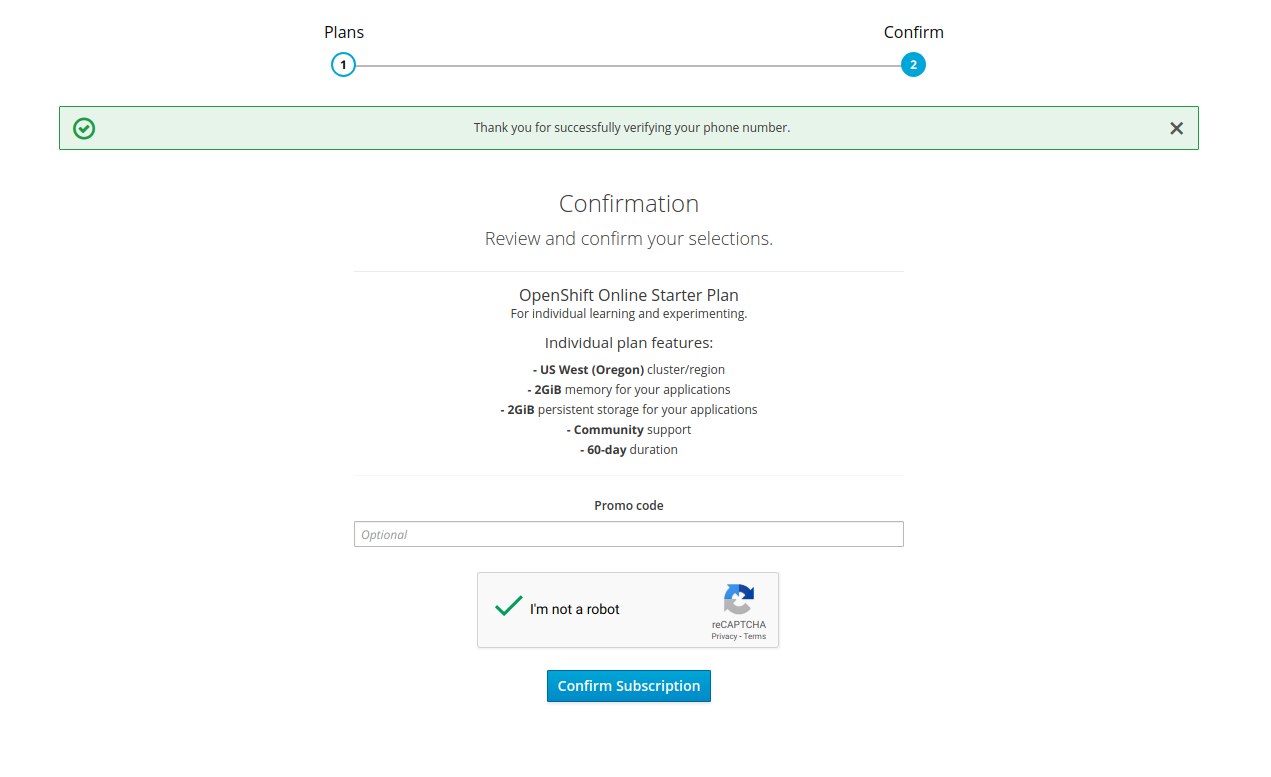
\includegraphics[width=0.9\linewidth]{img/os-overview}
	\caption{Übersicht des abgeschlossenen Plans}
	\label{fig:os-overview}
\end{figure}
Kurz nach dem Bestätigen sollte ein Bestätigungsmail eintreffen. Nach dem Bestätigen dieser kann bereits die Web Console geöffnet werden. Es wird ein Katalog mit allen Produkten von Openshift Online dargestellt (Abbildung \ref{fig:os-overview-catalog}).

\begin{figure}[h]
	\centering
	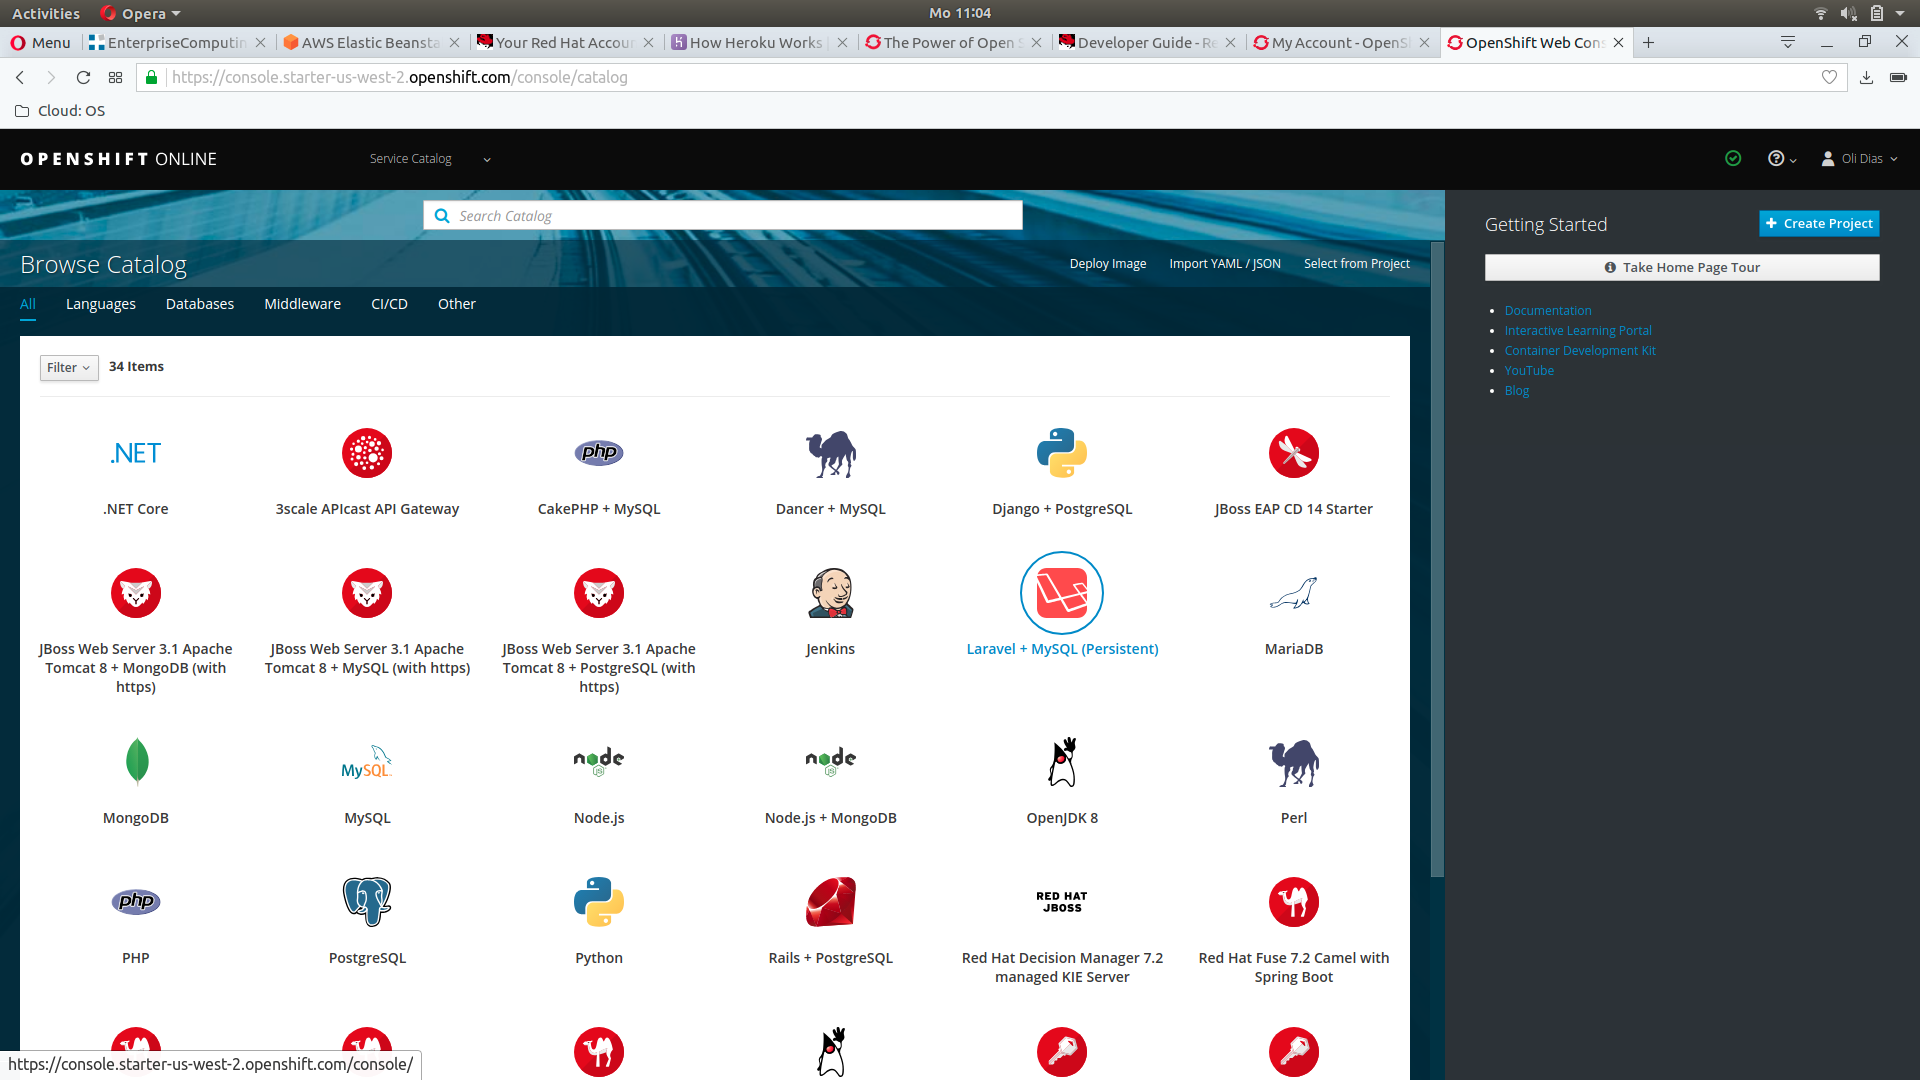
\includegraphics[width=0.7\linewidth]{img/os-overview-catalog}
	\caption{Katalog von Openshift}
	\label{fig:os-overview-catalog}
\end{figure}
Das Erstellen des Openshift Accounts ist somit abgeschlossen und die Plattform ist für das Builden und Deployen von Applikationen bereit. 
\subsubsection{Erstellen, Builden und Deployment der Applikation}
In der Web-Console können wir nun auf .NET Core Projekt clicken. Daraufhin erscheint ein Wizard, dem wir Schritt für Schritt folgen können. Falls das GitHub-Repository schon während dem Wizard hinzugefügt werden soll, muss es bereits existieren und sichtbar sein. 

Entsprechende Felder müssen gemäss Abbildung \ref{fig:os-new-config} ausgefüllt sein. Vorsicht ist bei der .NET Version geboten; wir verwenden die Version 2.2 von .NET Core. 
\begin{figure}[h]
	\centering
	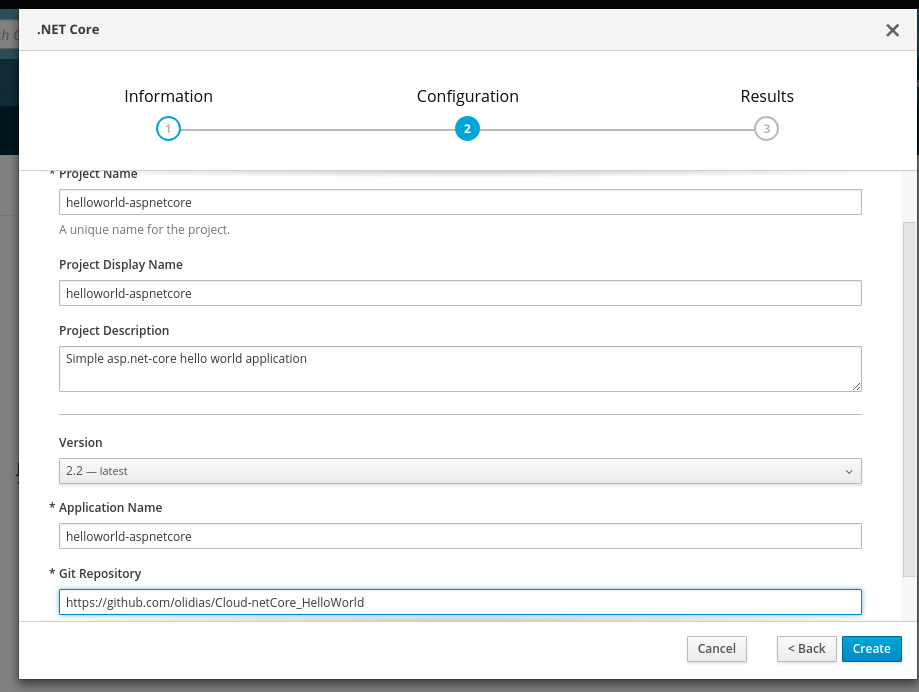
\includegraphics[width=0.7\linewidth]{img/os-new-config}
	\caption{Konfiguration des neuen Projektes}
	\label{fig:os-new-config}
\end{figure}

Sobald das Projekt in Openshift erstellt wurde, startet der Build. 
\begin{figure}[h]
	\centering
	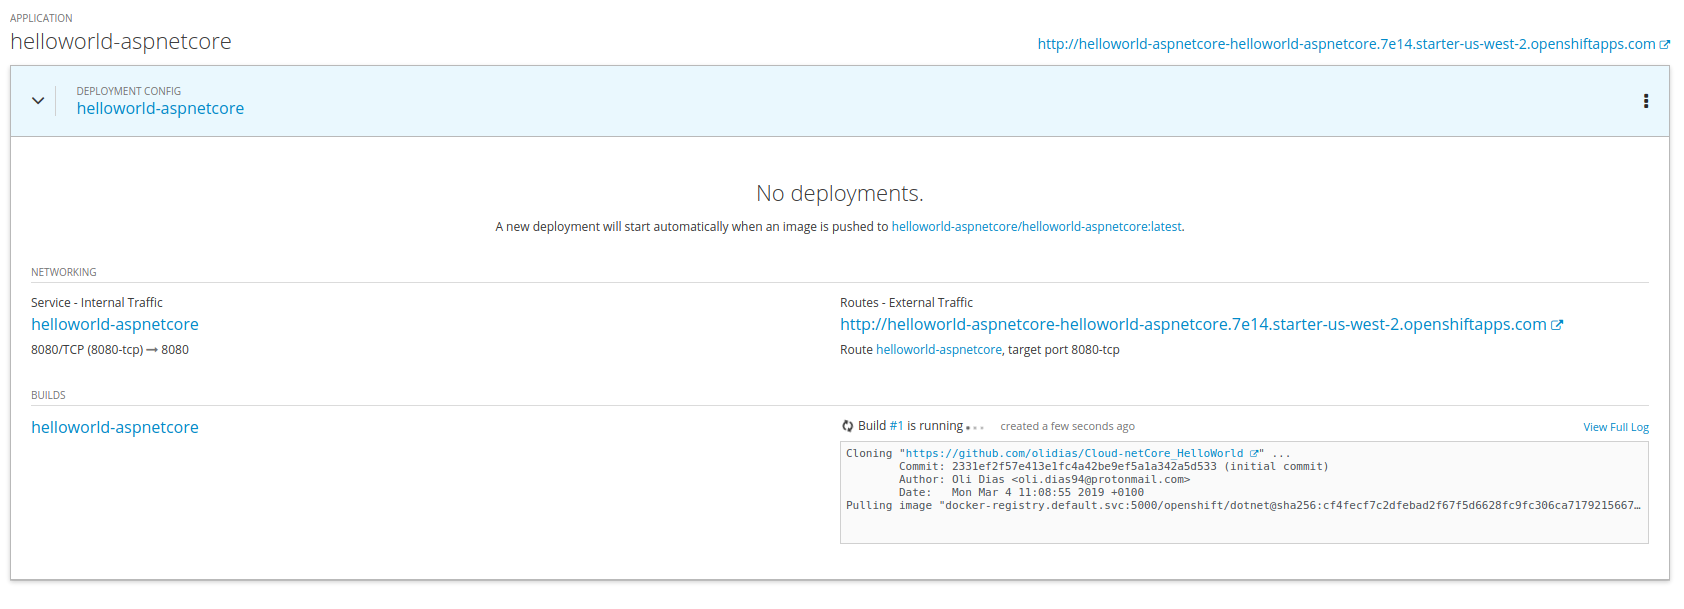
\includegraphics[width=0.7\linewidth]{img/os-building}
	\caption{Builden der .net core Applikation}
	\label{fig:os-building}
\end{figure}
Womöglich schlägt der Build aufgrund von fehlender \texttt{.s2i}-Konfiguration (Source-2-Image) fehl. Um diesen Fehler zu beheben, muss Openshift gesagt werden, wo das Startup-Projekt liegt. Dazu muss ein Ordner und File mit dem Namen \texttt{.s2i/environment} erstellt werden. Dies beinhaltet folgendes:
\begin{lstlisting}[breaklines=true]
DOTNET_STARTUP_PROJECT=HelloWorld-netcore/HelloWorld-netcore.csproj
\end{lstlisting}
Wichtig ist weiter zu beachten, dass die .net Versionen (dotnet sowie NuGet-Pakete) mit denjenigen von Openshift Cloud kompatibel sind. 

War der Build erfolgreich, muss noch das Deployment konfiguriert werden. Dazu kommt ein weiteres File mit dem Namen \texttt{run} ins \texttt{.s2i} Verzeichnis. Darin muss die Applikation noch gestartet werden. Dies funktioniert so:
\begin{lstlisting}
exec dotnet run
\end{lstlisting}
Ist auch dieser Schritt vollbracht, kann im Control Panel des Projektes zu Deployments $\rightarrow$ Routes navigiert werden. Dort erscheint eine Tabelle, wo der Hostname bereits angegeben ist und womit nun die Asp.Net-Core Applikation vom Internet her erreichbar ist.
\section{Analyse: OSSM-Definition}

Damit sich jemand als Cloud Computing Provider ausgeben kann, sollten folgende Chrakteristiken erfüllt sein:

\begin{itemize}
	\item On-demand
	\item Self-service
	\item Scalable
	\item Measurable
\end{itemize}

In den folgenden Kapiteln erläutern wir, wie Openshift diese umsetzt.

\subsection{On-demand \& Self-service}

Auf der Startseite findet man eine Katalog aller möglichen Projekttypen. Nach einem Klick auf den gewünschten Projekttyp erscheint ein Dialog, in welchem die spezifische Konfiguration vorgenommen werden kann. Gleichzeitig wird geprüft, ob die definierte Konfiguration plausibel ist. Ist dies der Fall, kann das Projekt erstellt werden.
Nach wenigen Sekunden ist das Projekt unter der Rubrik "My Projects" ersichtlich.

\begin{figure}[h]
	\centering
	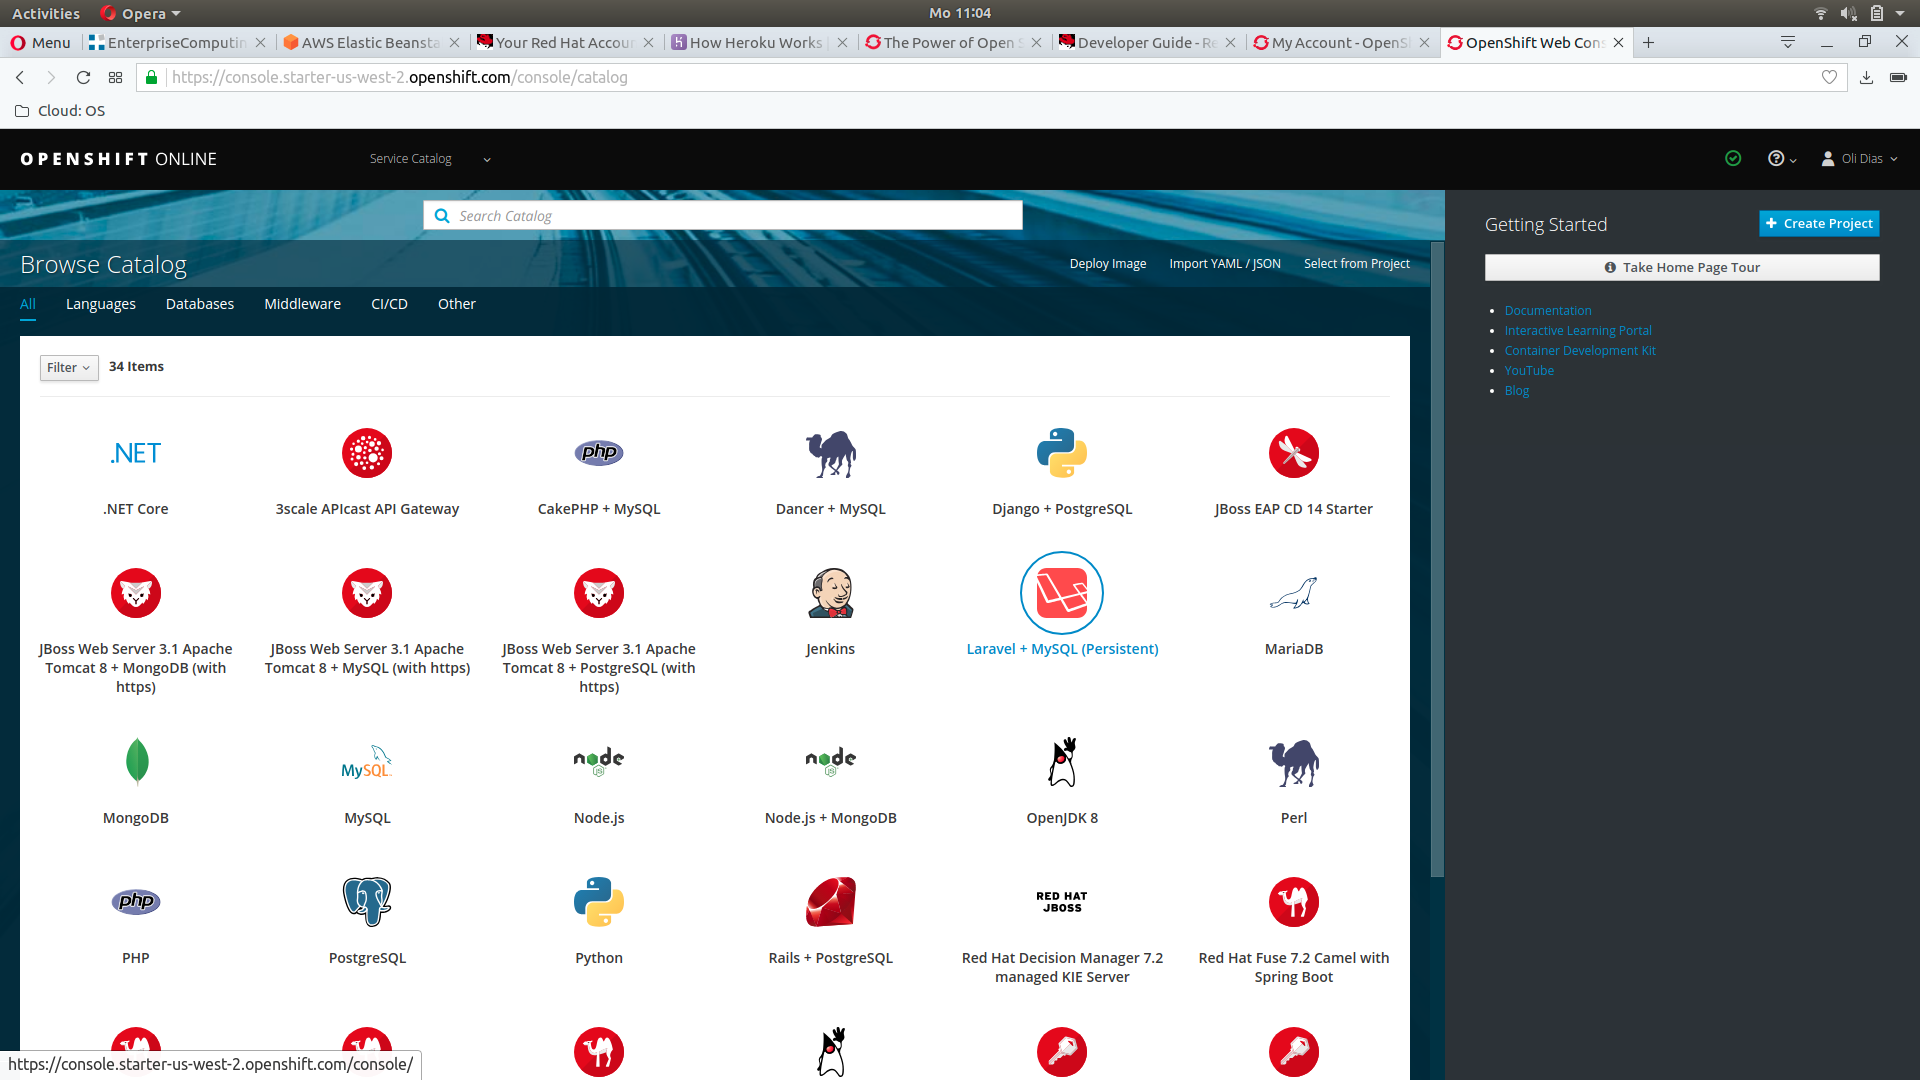
\includegraphics[width=0.7\linewidth]{img/os-overview-catalog}
	\caption{Auswahlkatalog aller möglichen Projekttypen}
	\label{fig:os-catalog}
\end{figure}

\begin{figure}%
    \centering
    \subfloat[label 1]{{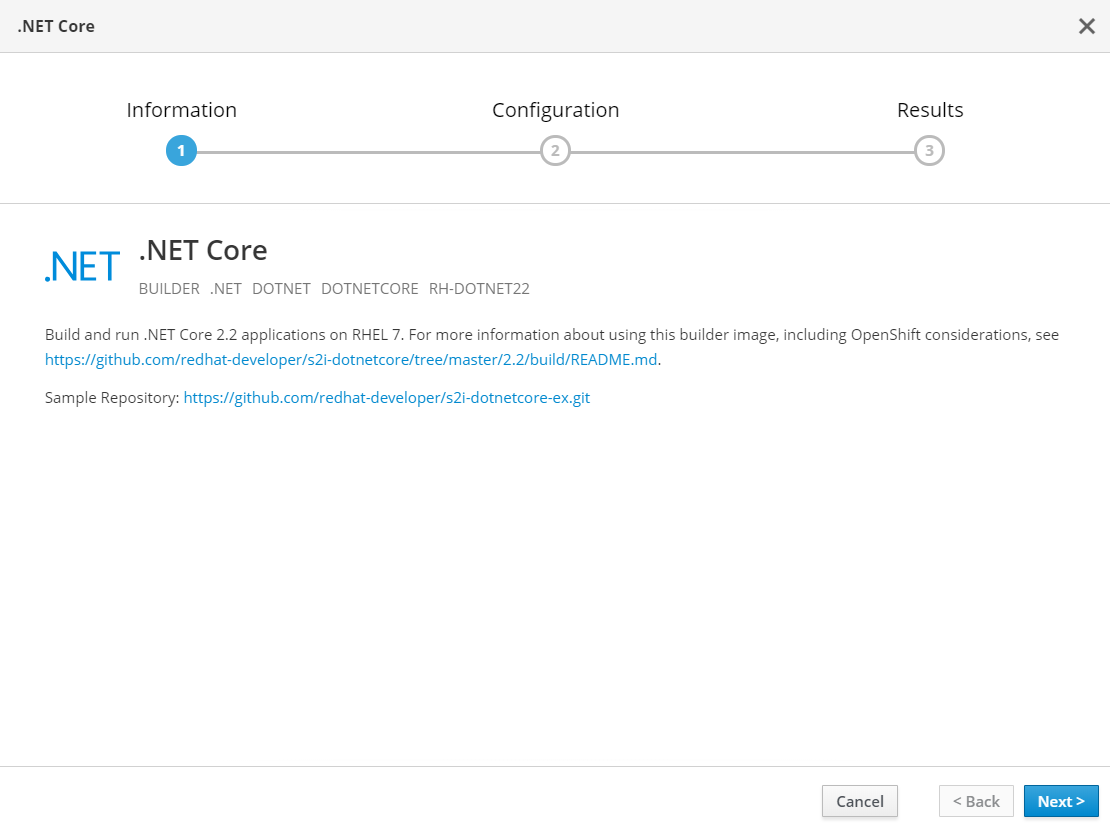
\includegraphics[width=5cm]{img/os-project-setup-1} }}%
    \qquad
    \subfloat[label 2]{{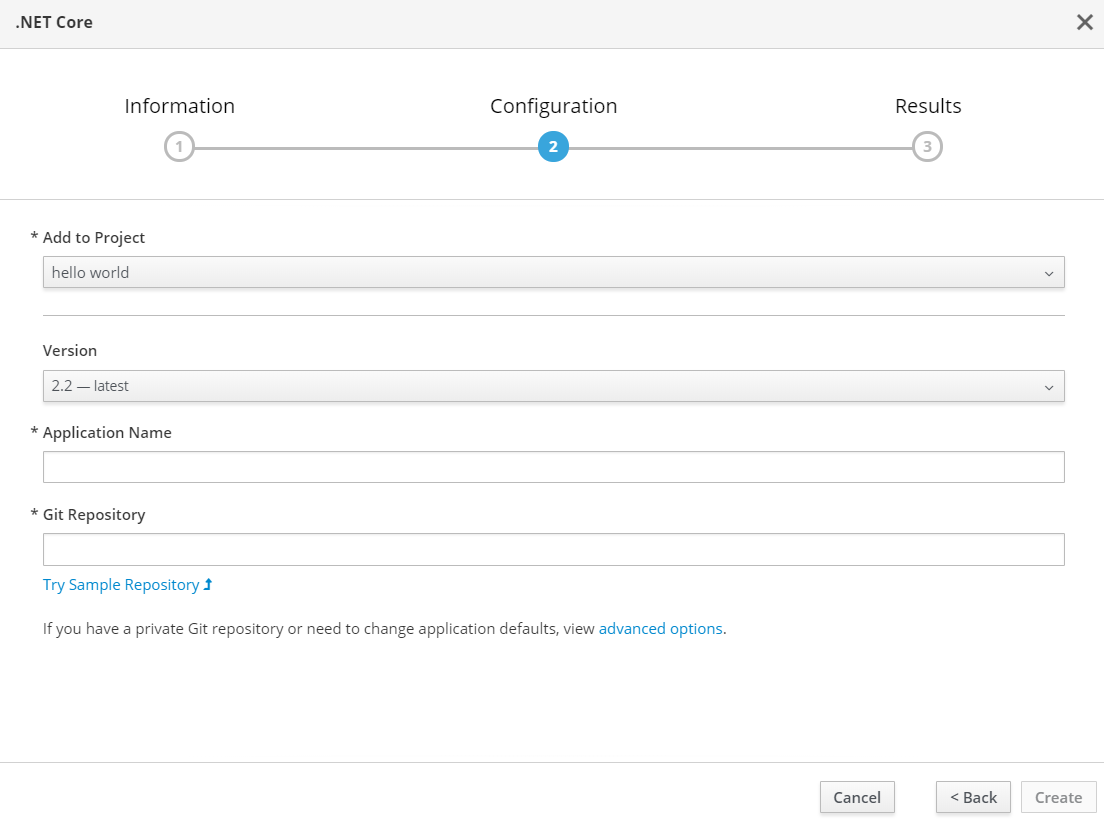
\includegraphics[width=5cm]{img/os-project-setup-2} }}%
    \caption{Setup Dialog}%
    \label{fig:os-setup}%
\end{figure}

Die Projektübersicht bietet nebst einigen generellen Informationen die Möglichkeit zum Build und Deployment.

\begin{figure}[h]
	\centering
	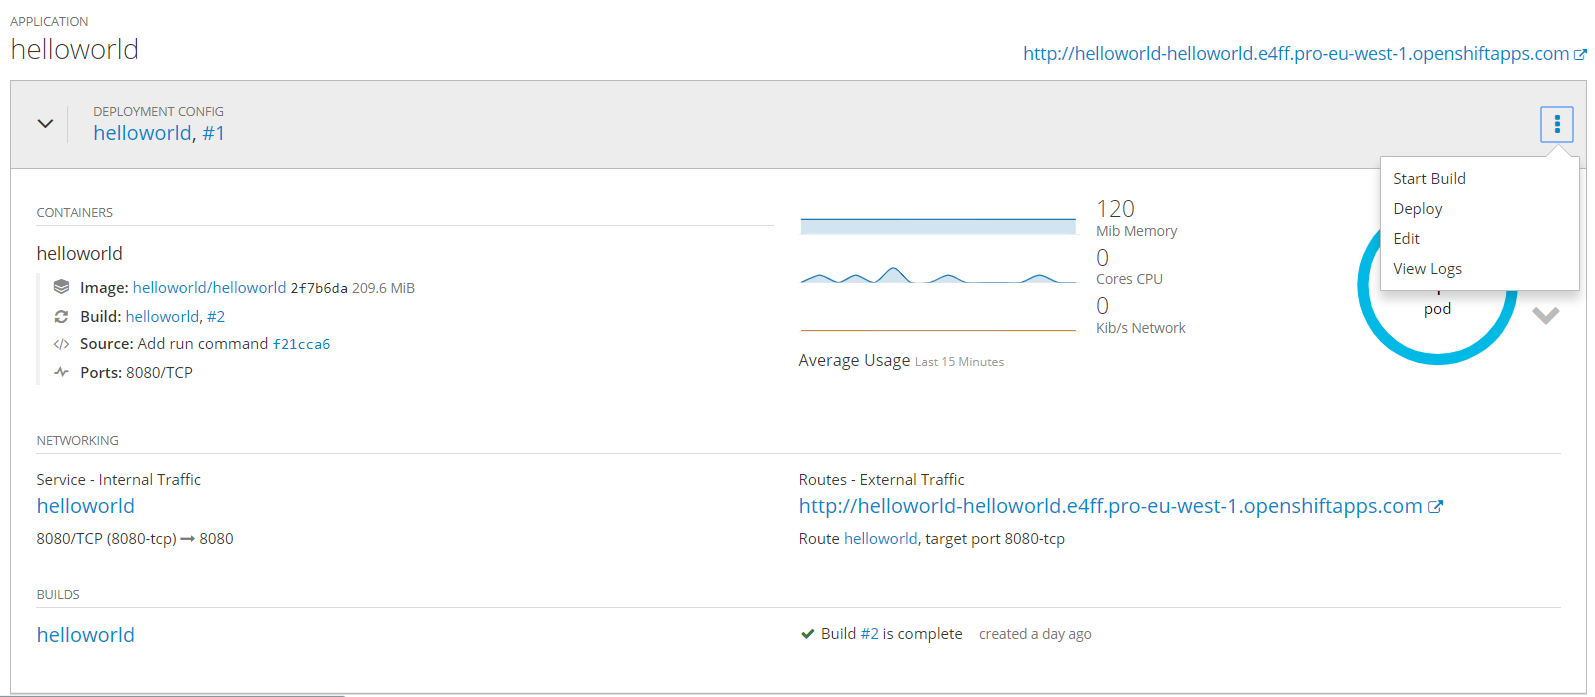
\includegraphics[width=0.7\linewidth]{img/os-project-overview}
	\caption{Ansicht der Projektübersicht}
	\label{fig:os-project-overview}
\end{figure}

\subsection{Scalable}

Die Nutzung von Openshift erfordert, dass man sich für ein Abonnement entscheidet. Nebst den kostenlosen Einführungsangeboten bedarf die langfristige Nutzung das Abonnement "OpenShift Online Pro". Im Standard bekommt man hierfür folgende Ressourcen:

\begin{itemize}
	\item 10 Projects
	\item 2 GB Memory
	\item 2 GB Terminating Memory
	\item 2 GB Storage
\end{itemize}

Um mehr als 10 Projekte zu verwalten bedarf es einem neuen Abonnement. Falls mehr Arbeitsspeicher oder Speicher nötig ist, kann das aktuelle Abonnement angepasst werden, was natürlich einen Einfluss auf den Preis hat. Trotzdem gibt es folgende Begrenzungen:

\begin{itemize}
	\item Arbeitsspeicher: maximal 48 GB
	\item Speicher: maximal 150 GB
\end{itemize}

\begin{figure}[h]
	\centering
	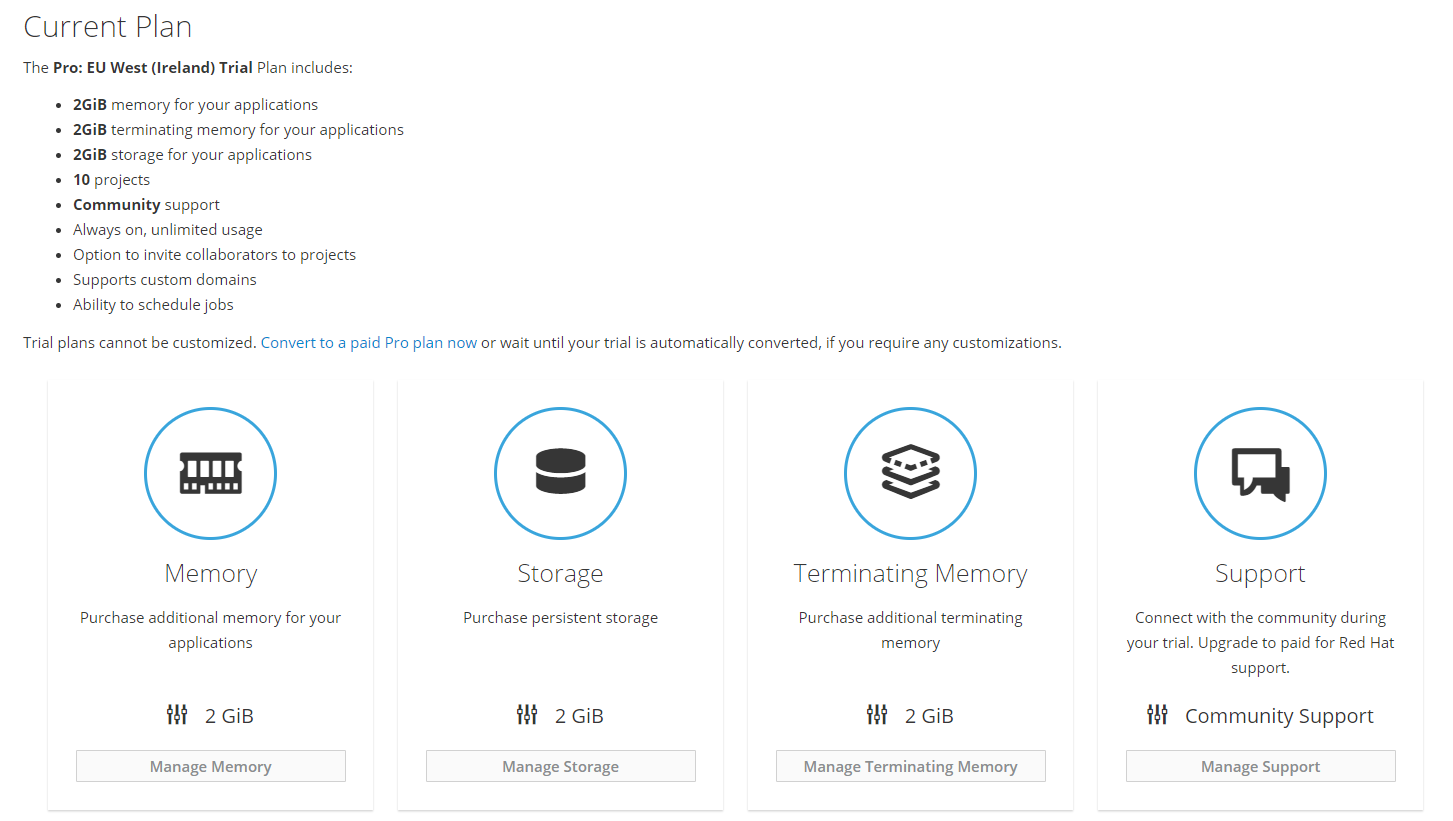
\includegraphics[width=0.7\linewidth]{img/os-scalability}
	\caption{Verwaltung der Ressourcen eines Abonnements}
	\label{fig:os-scalability}
\end{figure}

\subsection{Measurable}

Die aktuelle Nutzung der Ressourcen kann lediglich auf Projektstufe eingesehen werden. Diese Übersicht ist ziemlich einfach gehalten, ledicglich genutzer Arbeitsspeicher und Speicher werden im Verhältnis zum Maximum angezeigt.

\begin{figure}[h]
	\centering
	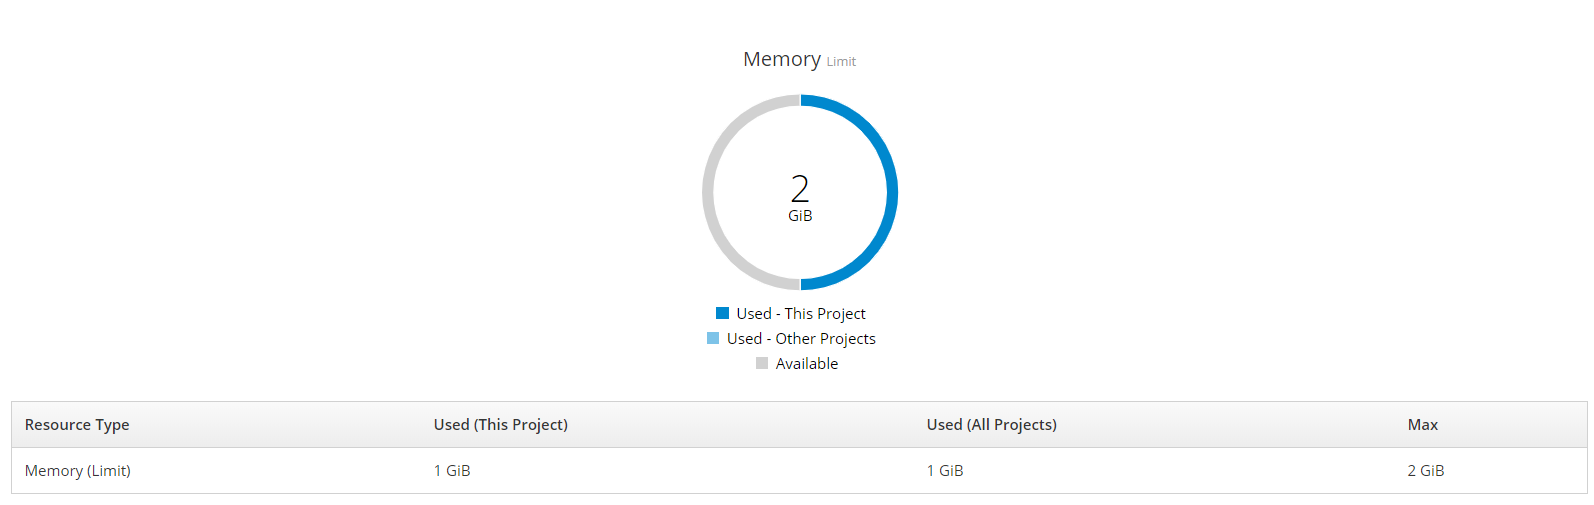
\includegraphics[width=0.7\linewidth]{img/os-quota}
	\caption{Übersicht der genutzten Ressourcen}
	\label{fig:os-quota}
\end{figure}

\section{Konzept: Cloud Computing Patterns}

Openshift bietet Entwicklern mit dem Konzept PaaS eine Plattform an, auf welcher eine App relative einfach deployed werden kann. Dies bringt den Vorteil, dass der Entwickler sich nicht mit der Komplexität der Building-/Deploying Infrastruktur auseinandersetzen muss.
Die Applikation läuft anschliessend auf sogenannten "Pods", welche vergleichbar mit Docker-Container sind. Einerseits kann die Anzahl Pod's pro Projekt manuell festeglegt und geändert werden. Zudem gibt es die Mgölichkeit für Pod Autoscaling. Sobald ein Pod bis zu
einem gewissen Grad ausgelastet wird, kommt ein zusätzlicher Pod in Aktion, sofern die maximale Anzahl definierter Pod's nicht erreicht wurde.

\begin{figure}[h]
	\centering
	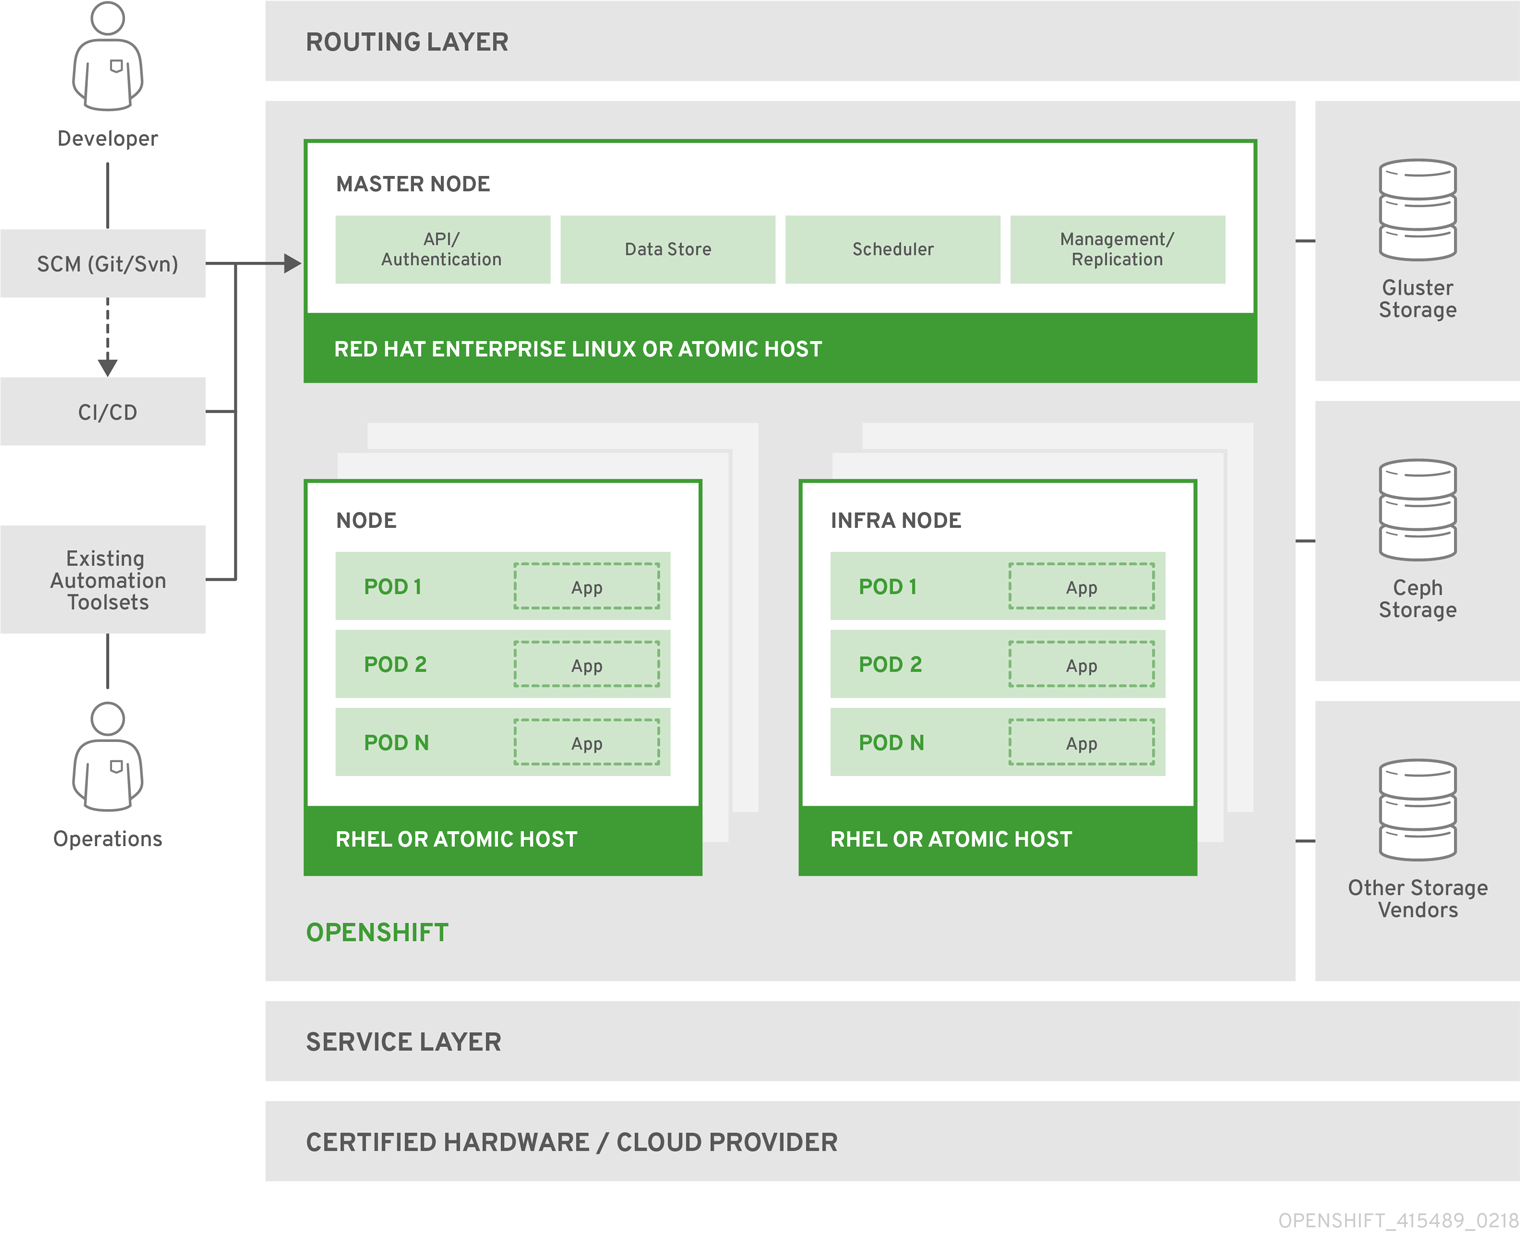
\includegraphics[width=0.7\linewidth]{img/os-architecture}
	\caption{Architekturübersicht der Openshift-Plattform}
	\label{fig:os-architecture}
\end{figure}

\section{Hands-On: Self Information}

\section{Analyse: Preisrecherche}

\section{Analyse: Preisvergleich eigenes Hosting, IaaS und PaaS}

\end{document}